\documentclass[handout]{beamer}

\input{../Vor2017glærur}

\title{Tölvunarfræði 2}
\subtitle{Vika 2}

\begin{document}

\begin{frame}
\titlepage
\end{frame}

% \section{Inngangur að bendum}
% 
% \begin{frame}{Bendar}
% \begin{itemize}
%  \item Bendir er breyta sem inniheldur staðsetningu minnissvæðis
%  \begin{itemize}
%   \item Hún ``bendir á'' minnissvæðið
%  \end{itemize}
%  \item Hægt er að nota bendinn til að fá aðgang að gögnunum sem geymd eru í minnissvæðinu
% \end{itemize}
% \begin{center}
% 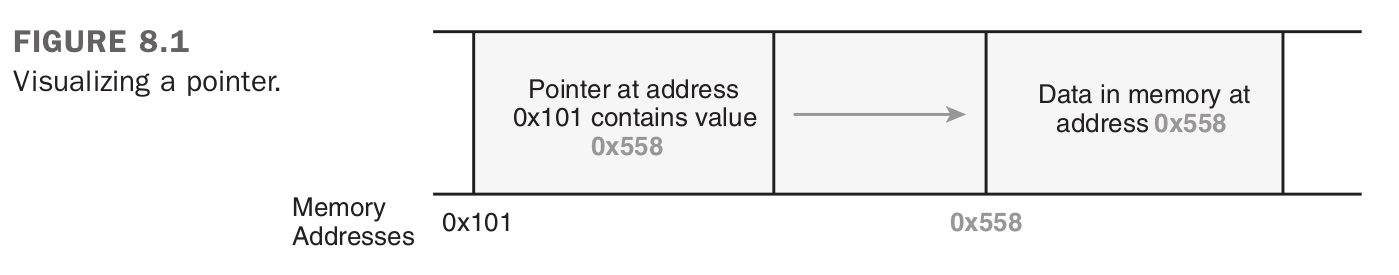
\includegraphics[width=\textwidth]{pointer-visualization}
% \end{center}
% \end{frame}
% 
% \begin{frame}[fragile]{Bendar}
% Við búum til bendi sem vísar á breytu af gerðinni \texttt{gerd} með \texttt{gerd*}. Við náum í staðsetningu minnissvæðis með \texttt{\&} virkjanum.
% \cppfile[firstline=6, lastline=10, gobble=4, fontsize=\small, label=pointerintro.cpp]{Code/w1/pointerintro.cpp}
% \end{frame}
% 
% \begin{frame}[fragile]{Bendar}
% Við getum sótt gögn sem bendir vísar á með \texttt{*} virkjanum.
% \cppfile[firstline=6, lastline=15, gobble=4, fontsize=\small, label=dereferencing.cpp]{Code/w1/dereferencing.cpp}
% \end{frame}

\section{Breytur og minni í C++}

\begin{frame}{Líftími breyta}
\begin{itemize}
 \item Við munum að breytur hafa mismunandi líftíma
 \begin{itemize}
  \item Aðskilið hugtak: gildissvið breytu (e. \emph{variable scope})
 \end{itemize}
 \item Í C++ getur líftími breytu verið af nokkrum gerðum, þá helst
 \begin{itemize}
  \item Sjálfvirkur (e. \emph{automatic}) - líftími breytunnar er ákvarðaður sjálfkrafa
  \item Kyrrstæður (e. \emph{static}) - breytan lifir meðan forritið keyrir
  \item Kvikstæður (e. \emph{dynamic}) - breytan lifir meðan forritari segir
 \end{itemize}
 \item Í flestum forritunarmálum sem við erum líkleg til að hafa skoðað hingað til sér ruslasafnari (e. \emph{garbage collector}) um að hreinsa til, en venjulegt C++ hefur ekki slíkan
\end{itemize}
\end{frame}

\begin{frame}{Minnissvæði í C++}
\begin{itemize}
 \item Í keyrandi C++ forriti eru (venjulega) nokkrar gerðir minnis í gangi á hverjum tímapunkti
 \begin{itemize}
  \item Þula (e. \emph{code segment}). Geymir upplýsingar um forritið - vélamálsskipanir og fasta, venjulega er eingöngu lesaðgangur
  \item Gagnasvæði (e. \emph{data segment}).
  Frátekið í upphafi keyrslu, getum ekki stækkað eða minnkað.
  \item Hlaði (e. \emph{stack}). Minnissvæði af breytilegri stærð sem hægt er að fá aðgang að á skipulegan máta
  \item Kös (e. \emph{heap}). Er úthlutað og skilað að beiðni forritsins, minnisdreifing ekki endilega mjög fyrirsjáanleg
 \end{itemize}
 \item Hlaðinn og kösin eru þau svæði sem við þurfum að skoða sérstaklega
\end{itemize}
\end{frame}

\begin{frame}{Hvað fer svo hvert?}
\begin{itemize}
 \item Þumalputtareglur fyrir ``venjulegt'' C++
 \begin{itemize}
  \item Líftími staðværra (e. \emph{local}) breyta er ákvarðaður sjálfkrafa og þær eru settar á hlaðann
  \item Víðværar (e. \emph{global}) breytur og breytur skilgreindar sem \texttt{static} fara í gagnasvæðið
  \item Kvikstæðar breytur fást með sérstökum minnisúthlutunaraðgerðum eins og \textbf{new} og eru settar í kös
 \end{itemize}
\end{itemize}
\end{frame}

\begin{frame}{Hlaðinn}
\begin{columns}
\column{0.6\textwidth}
\begin{itemize}
 \item Hlaðinn er ``lítið'' minnissvæði sem C++ forrit nota til að halda utan um staðværar breytur og upplýsingar um fallsköll
 \begin{itemize}
  \item Getum lent í því að hlaðinn fyllist
 \end{itemize}
 \item Uppbygging er skipuleg (LIFO)
 \begin{itemize}
  \item Hentar vel fyrir raunverulega örgjörva, gerir mjög hraða vinnslu mögulega
 \end{itemize}
 \item Líftíma breyta á hlaðanum er stjórnað sjálfkrafa í C++, minninu er skilað þegar viðkomandi fall skilar af sér
\end{itemize}
\column{0.4\textwidth}
\begin{center}
Uppbygging hlaðans

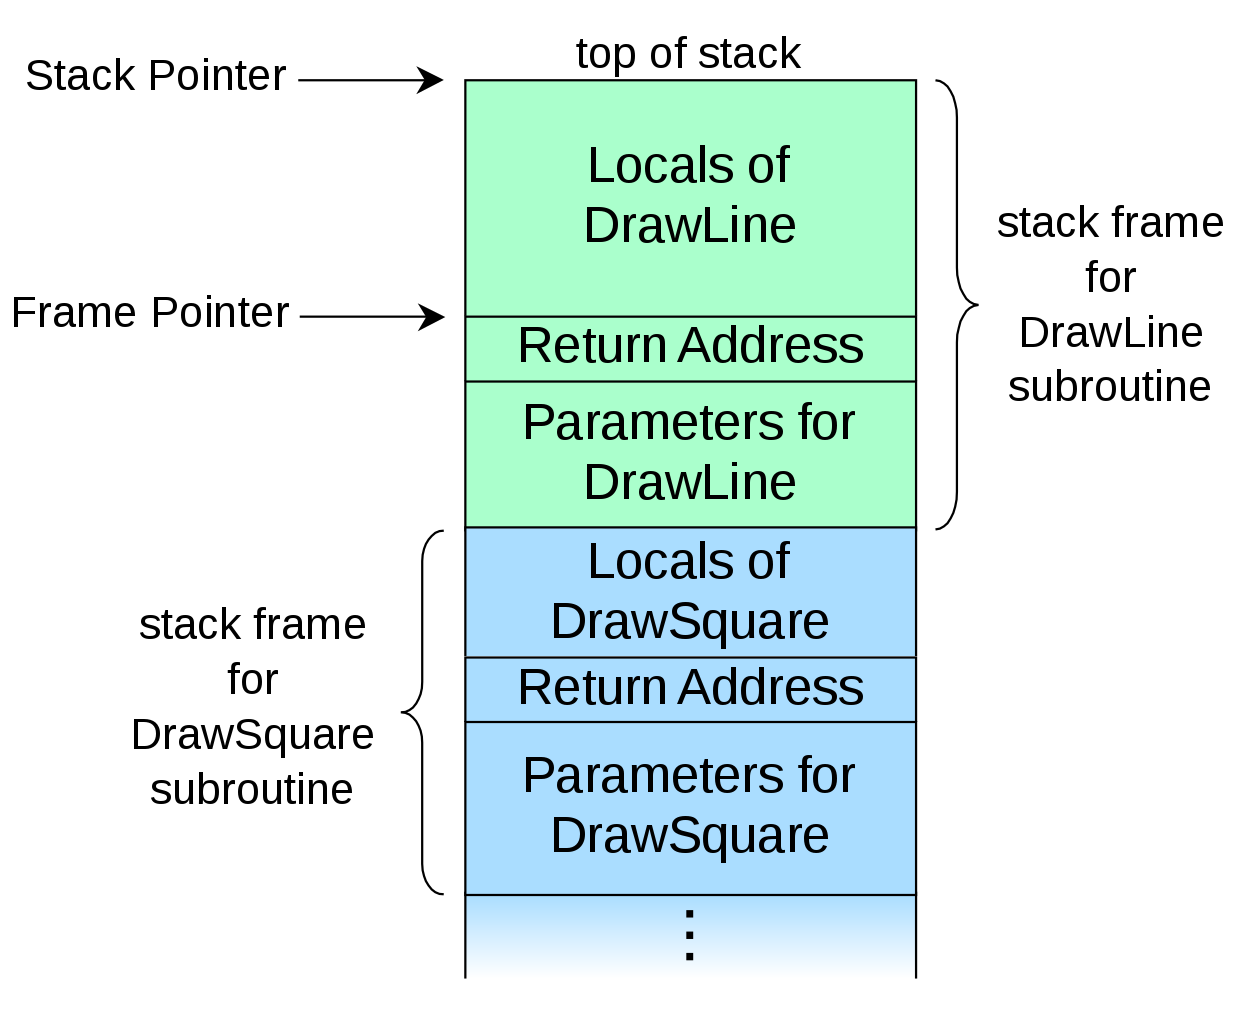
\includegraphics[width=\linewidth]{call-stack-layout}

{\tiny Mynd: \href{https://en.wikipedia.org/wiki/File:Call_stack_layout.svg}{Wikimedia}}
\end{center}
\end{columns}
\end{frame}

\begin{frame}{Kösin}
\begin{columns}
\column{0.7\textwidth}
\begin{itemize}
 \item Kösin er ``stórt'' minnissvæði sem C++ forrit geta beðið um skerf af á keyrslutíma
 \item Er ekki endilega samfellt, getur verið mjög uppskipt (e. \emph{fragmented})
 \item Hægur aðgangur í samanburði við aðgang að hlaðanum
 \item Hægt er að fá aðgang að kösinni hvaðan sem er úr forritinu
 \begin{itemize}
  \item Takmarkast ekki við fallskall
 \end{itemize}
 \item C++ forrit sem fær aðgang að kös með \texttt{new} þarf að skila svæðinu með \texttt{delete}
\end{itemize}
\column{0.3\textwidth}
\begin{center}
Vond uppskipting

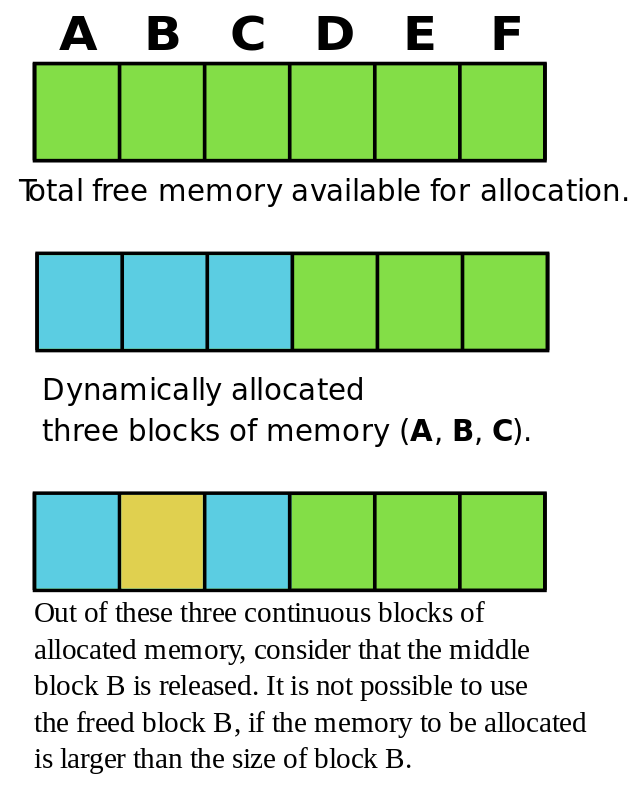
\includegraphics[width=\linewidth]{external-fragmentation}

{\tiny Mynd: \href{https://commons.wikimedia.org/wiki/File:External_Fragmentation.svg}{Wikimedia}}
\end{center}
\end{columns}
\end{frame}

\begin{frame}{Að setja hluti í kös}

\end{frame}

\begin{frame}{Notkun viðfanga í C++}

\end{frame}


\section{Hlutbundin forritun í C++}

\subsection{Helstu hugtök í hlutbundinni forritun}




\section{Lokaorð}

\begin{frame}{Þessi glærupakki}
Tengill á fyrirlestraræfingu: \url{https://goo.gl/forms/qaB2Hoxwd6PFEN9I2}
\vspace{1cm}

Öll nafngreind forrit í þessum glærupakka, ásamt glærupakkanum sjálfum, má finna á  \href{https://github.com/Ernir/kennsluefni/tree/master/T2/Code/w1}{Github}.

\end{frame}


\begin{frame}{Næst}
Frekari forritun í C++, staðalsafnið.
\end{frame}


\end{document}
